
\begin{figure}[H]
  \centering
  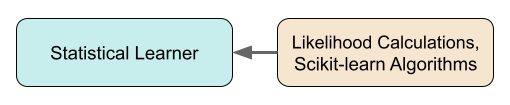
\includegraphics[width=0.7\linewidth]{./chapters/exp1/methodology3.png}
  \caption{Third portion of the flowchart from Figure \ref{fig:method} being 
           described in this section.}
\end{figure}

Choosing which algorithms to test is largely intuitive, but since this work has
yet to be benchmarked with simple algorithms, two straightforward algorithms
were chosen, \textit{k}-nearest neighbors and decision trees, and were
introduced in Section \ref{sec:algs}. Also covered in that section is the
mathematical framework of the \gls{MLL} calculation method. The implementation
details of these three approaches are covered here. 

\subsection{Scikit-learn Algorithms}

The machine learning toolkit chosen for this work is scikit-learn
\cite{scikit}, a package in python.  Virtually all modern \gls{ML} toolkits
will have acceptably fast and reliable algorithms, but the use of python
provides a platform for seamless integration of all the tools in the workflow.
This section walks through the implementation of the two scikit algorithms. 

\todo[inline]{warning: discuss training set scaling}
\todo[inline]{is more detail, i.e. code snippets from scripts, needed?}

The first step is splitting the training set into the features ($X$, with 29
nuclide mass measurements), and a single set of labels ($y$, e.g., burnup).
Next, the two algorithms are initialized.  The labels that require regression
analysis (burnup, enrichment, cooling time) are predicted using the
\texttt{KNeighborsRegressor} and \texttt{DecisionTreeRegressor} in
scikit-learn. The reactor type label uses classifiers:
\texttt{KNeighborsClassifier} and \texttt{DecisionTreeClassifier}.  Each
algorithm has a list of hyperparameters that impact the model complexity and
prediction performance, as discussed in Section \ref{sec:complexity}. Since
this work is a demonstrative investigation, many of the default choices are
retained. However, some of these were tuned using hyperparameter optimization,
shown in Table \ref{tbl:exp1hypparam}.  The choices for each of these
algorithms is summarized below (note this is just a subset of all available
hyperparameters \cite{scikit}):
\todo[inline]{describe optimization in detail or no?}

\begin{enumerate}
  \item \texttt{KNeighborsClassifier} \& \texttt{KNeighborsRegressor}
    \begin{itemize}
      \item Number of nearest neighbors (\textit{k}) to include changes for 
            each prediction category and is in Table \ref{tbl:exp1hypparam}.
      \item Sample weighting is with respect to distance and not uniform.
      \item Distance metric is "Manhattan" (aka L1 loss, or absolute 
            differences).
    \end{itemize}
  \item \texttt{DecisionTreeClassifier} \& \texttt{DecisionTreeRegressor}
    \begin{itemize}
      \item Maximum number of features included is the length of the feature 
            set: 29.
      \item Maximum depth of decision tree changes for each prediction category
            and is in Table \ref{tbl:exp1hypparam}.
      \item For the classifier, the \texttt{class\_weight} is "balanced", 
            meaning that the weights are inversely proportional to the frequency
            of each class (\gls{PWR}, \gls{BWR}, \gls{PHWR}) in the training set.
      \item For both the classifier and regressor, the default splitting criterion
            (function for measuring the quality of a split) is kept. This is the 
            Gini impurity for the former, and mean squared error (aka L2 loss) 
            for the latter.
    \end{itemize}
\end{enumerate}

\begin{table}[!hbt]
  \centering
  \begin{tabular}{@{}lcll@{}}
  \toprule
    \textbf{\begin{tabular}[c]{@{}l@{}}Prediction\\ Parameter\end{tabular}}
  & \textbf{\begin{tabular}[c]{@{}l@{}}\textit{k} \\ (N neighbors)\end{tabular}}
  & \textbf{\begin{tabular}[c]{@{}l@{}}Max \\ Depth\end{tabular}}
  & \textbf{\begin{tabular}[c]{@{}l@{}}Max \\ Features\end{tabular}} \\ 
  \toprule
  Reactor Type & 4                 & 56        & 29           \\
  Burnup       & 1                 & 77        & 29           \\
  Enrichment   & 2                 & 45        & 29           \\
  Cooling Time & 1                 & 73        & 29           \\ \bottomrule
  \end{tabular}
  \caption{Optimized algorithm hyperparameters for the 29 nuclide mass training 
           set.}
  \label{tbl:exp1hypparam}
\end{table}

After the algorithms are initialized, the training set iteratively undergoes
error injection according to the method in Section \ref{sec:inforeduc1}. Next,
the (information reduced) data set is preprocessed by scaling and normalization
because the nuclide concentrations vary by many orders of magnitude. After
this, the training data features have a zero mean and unit variance. The
initialized algorithm is then used to fit the training set and is then ready
for prediction of "unseen" test samples.

Introduced in Section \ref{sec:testerr}, these algorithms provide predictions
based on the \textit{k}-fold \gls{CV} approach, not to be confused with the
\textit{k} in \textit{k}-nearest neighbors.  Tested were 5, 10, and 15 \gls{CV}
folds and they all performed the same because the training set is large.  Given
the equal performance among several options, the number of \gls{CV} folds was
chosen to be 5 based on computational expediency. The \texttt{KFold}
cross-validator with observation shuffling (i.e., the data set was shuffled
prior to splitting) in the scikit package carried out this task for the
regression prediction cases.  For reactor type classification, the
\texttt{StratifiedKFold} cross-validator was used since there is an imbalance
of classes in the training database.  \todo[inline]{do I have to prove they all
performed the same?} 

Because the performance needs to be compared to the \gls{MLL} predictions, the
scikit method \texttt{cross\_val\_predict} was used, as it returns the
predictions of each \gls{CV} fold as it becomes the test set. Thus, the entire
training set becomes a test case at some point, and the predictions return
equal the number of entries in the training set.

The scripts written to run the scikit-learn algorithms were deployed using
\gls{UW}-Madison's \gls{CHTC} resources and the \gls{UW} campus grid. 

\subsection{Maximum Log-Likelihood Calculations}

The \gls{MLL} calculation method is implemented in python using the SciPy
statistics toolkit and NumPy functionality \cite{scipy, numpy}. In this method,
one test sample is removed from the training set at a time, and the
log-likelihood calculation in Equation \ref{eq:loglike} is performed between
the test sample and all the rows of the training set.  The observation with the
largest log-likelihood is returned as the predicted labels. Just like with the
scikit-learn algorithm-based predictions, the entire training set becomes a
test sample at some point, so the predictions returned equal the number of
entries in the training set.

A key difference in how the \gls{MLL} method provides predictions is that it
returns all the labels together, so it is not doing any generalizing on the
continuous variable labels (burnup, enrichment, and cooling time). It is
analogous to \textit{k}-nearest neighbors where $k = 1$, because there is no
model being created, it just matches upon the call for prediction. Because of
this, the \gls{MLL} method performing well is highly dependent on the training
set being sufficiently large. 

The scripts written to run the \gls{MLL} calculations were deployed using
\gls{UW}--Madison's \gls{CHTC} resources, the \gls{UW} campus grid, and the 
\gls{OSG} \cite{osg07, osg09}. 
